\section{Proposed method}\label{sec:yourmethod}

This section defines the scope of our implementation, describes our initial baseline
implementation, analyzes its bottlenecks and outlines the steps which were followed to
increase performance.

\mypar{Scope} In our project, we focus on grayscale images of size $s \times s$,
where $s$ is a power of two. The quadtree partitioning has the maximum depth $m$
and the error threshold $\epsilon$ as parameters. To simplify vectorization, we
also ensure that the range blocks do not get smaller than $4 \times 4$ pixels.
Furthermore, exhaustive block mapping to search for suitable transformations is
used. Our focus is solely on compression, which is the performance bottleneck in
fractal image compression.

\mypar{Baseline implementation}
The baseline is written from scratch in C. Algorithm~\ref{alg:baseline} illustrates the compression of the algorithm,
whose inputs are the image (row-wise array of doubles) of size $s \times s$, the max quadtree depth $m$ and the error threshold $\epsilon$.

The function \texttt{partition(image,s)} partitions the image into contiguous non-overlapping blocks of size $s \times s$.
The function \texttt{quad($R_i$,s)} takes a range block of size $s \times s$ and partitions it into 4 smaller range blocks.
The function \texttt{compute(image,$R_i$,$D_i$)} computes a transformation with its resulting RMS according to section~\ref{sec:background}.
This function also downscales the domain block to the size of the range block, rotates it three times (90, 180 and 270 degrees)
and returns the best of the four possible transformations.
\begin{algorithm}
\caption{Compression using iterative quadtree partitioning}\label{alg:baseline}
\hspace*{\algorithmicindent} \textbf{Input:} \texttt{img}, $\epsilon$, $m$ \\
\hspace*{\algorithmicindent} \textbf{Output:} $\boldsymbol{T}$ (set of computed transformations)
\begin{algorithmic}[1]
  \State $\boldsymbol{T} \gets \{\}$
  \State $\boldsymbol{R} \gets $ \Call{partition}{\texttt{img}, $s/2$}
    \For{$c=1..m$}
        \State $\boldsymbol{D} \gets $ \Call{partition}{\texttt{img}, $s/2^{c-1}$}
        \For{$R_i \in \boldsymbol{R}$}
            \State $err_i \gets \infty, T_i \gets \NULL$
            \For{$D_i \in \boldsymbol{D}$}
              \State $T_x, err_x \gets $ \Call{compute}{\texttt{img}, $D_i$, $R_i$}
              \If{$err_x < err_i$}
                \State $T_i \gets T_x$
                \State $err_i \gets err_x$
              \EndIf
            \EndFor
        \EndFor
        \State $\boldsymbol{R} \gets \boldsymbol{R} \backslash  R_i$
        \If{$err_i > \epsilon$}
          \State $\boldsymbol{R} \gets \boldsymbol{R} \cup  \Call{quad}{R_i, s/2^c}$
        \Else
          \State $\boldsymbol{T} \gets \boldsymbol{T} \cup \{T_i\}$
        \EndIf
    \EndFor
\end{algorithmic}
\end{algorithm}

As opposed to algorithms in \cite{fisher2012} and \cite{github-cpp}, this algorithm does not implement quadtree
partitioning recursively but iteratively.
Our optimized versions (see later) depend heavily on precomputations of domain blocks (especially downscaling).
At every quadtree depth, the domain blocks shrink with the range blocks. At every quadtree depth $c$ we have a pool of
domain blocks $D^{(c)}$. In an iterative approach, we can perform precomputations on $D^{(c)}$, process all domain/range block pairs
and then discard the precomputations. Using a recursive approach, all precomputations of all domain block pools must be kept in memory
to avoid recomputing the precomputations.

\mypar{Roofline} We used the roofline model \cite{applying-roofline} to see
whether the algorithm is memory or compute bound. The peak performance $\pi$ was
determined by counting the dispatch ports specified in Intel's
\texttt{Optimization Reference Manual} \cite{intel-opt-manual}. We distinguish
between scalar and vectorized peak performance. The bandwidth $\beta$ was
measured with the STREAM benchmark \cite{stream}. We verified both the peak
performance and the bandwidth with the Empirical Roofline Tool \cite{ert}, which
confirmed the values.

For the program model, we need to measure the work $W$, the runtime $T$ and the
data move movement $Q$ of the algorithm. Due to the dynamic nature of quadtree,
the model does not only depend on the image size but also on the content of the
image itself. Therefore, we define the three quantities as $W=W(s, img)$,
$T=T(s, img)$ and $Q=Q(s, img)$, where $s$ and $img$ are defined as in
algorithm~\ref{alg:baseline}. We measured $W$ by instrumenting the code
according to the cost metric in equation~\eqref{eq:cost}. For measuring $T$, we
used the \texttt{RDTSC} instruction available on all x86 architecture and
disabled Turbo Boost to guarantee an integer runtime. The measurement of $Q$ is
the most challenging and requires performance counters which are not supported
by our hardware. A correct, yet too pessimistic lower bound for $Q$ is
$Q \geq 8 \cdot s^2$ because we have to load the image (at least) once from
memory. One of our group members developed a tool to simulate a program's memory
accesses throughout the course, supporting multi-level caches
\cite{github-cache}.

We simulated our scalar-optimized code with this tool for the hardware we run our benchmarks on,
which should give us a tighter lower bound for $Q$.
This simulation is still too pessimistic for the non-optimized code but more accurate for our scalar-optimized and vectorized code.
Our experiments showed that for small images ($\leq 512 \times 512$), our theoretical bound holds well.
It is no surprise that for larger images ($\geq 1024 \times 1024$) the theoretical bound is way too pessimistic
because these images do not entirely fit into L3 cache of our hardware anymore, which leads to more traffic between main memory and cache.

To place the baseline in the roofline plot, we calculated the operational
intensity $I=\frac{W}{Q}$ and the performance $P=\frac{W}{T}$ of our
implementation. Figure \ref{fig:roofline} shows the roofline plot for a specific
image with different sizes. One can see that the baseline is inherently compute
bound and we have good potential for performance improvement as the baseline
runs only at 12.5\% of scalar peak performance. Next, we use profiling to find
the performance bottlenecks of the code.

\begin{figure}
  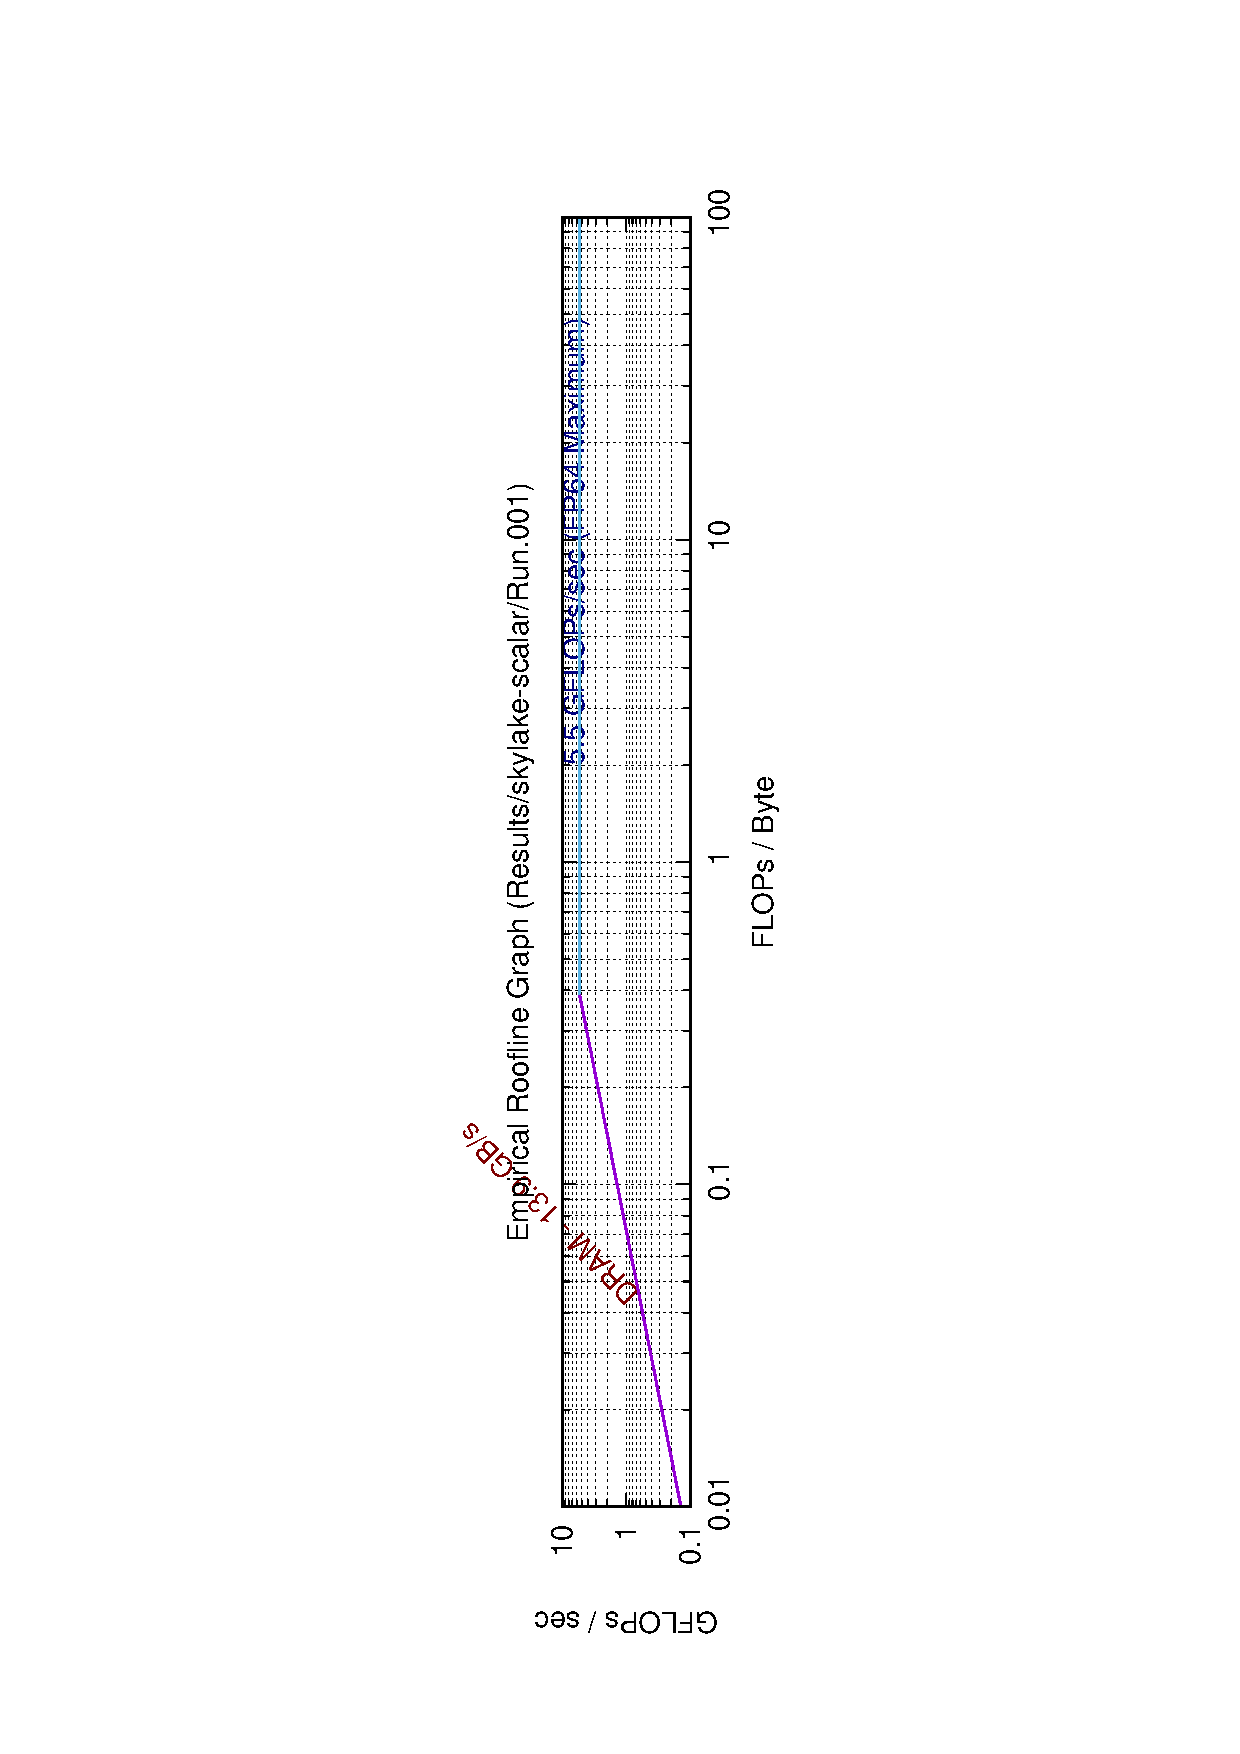
\includegraphics[page=1, width=.45\textwidth]{roofline}
  \caption{Roofline plot for the baseline and various performance optimizations}
  \label{fig:roofline}
\end{figure}

\mypar{Hotspots} A major performance blocker is the exhaustive search for block matches.
In our project, we focus solely on performance,
whereas using a better search strategy as mentioned in section \ref{sec:intro} is an algorithmic improvement
and thus out of scope in the project.

When inspecting the code of the baseline, it is apparent that the majority of the work
is done when calculating the contrast, brightness and error of each range/domain block pair
(equations \ref{contrast}, \ref{brightness} and \ref{error}). We used \textit{Valgrind}
\cite{valgrind} to profile the code and the profiling report confirmed our assumption. Especially, the sums
over all pixels of a block were identified as hotspots so we started our optimizations there.

\mypar{Scalar Optimizations} As a first optimization we moved the calculation of the sums $\sum_{i=1}^n a_i$,
$\sum_{i=1}^n a_i^2$, $\sum_{i=1}^n b_i$ and $\sum_{i=1}^n b_i^2$ out of the nested loop
(see algorithm \ref{alg:baseline} line 5 and 7). The values of these sums change only if the algorithm advances
to the next quadtree depth so we can easily precompute them in each quadtree iteration and reuse them when we
compare each domain block with a range block.

The baseline implementation focuses on a clear and understandable code style. Therefore, it uses a queue
to keep track of the remaining range blocks and several structs to model different concepts of the algorithm
(e.g. the image and domain/range blocks). More precisely, a block is a struct with integer coordinates $x,y$ and a size $s$.
Both the queue and the usage of structs are not optimal for performance so we replaced them
with simple variables and arrays. With this change, we went from \textit{explicit} to \textit{implicit} blocks.
A block at quadtree depth $m$ can be uniquely identified by an index $i$. Its size $s$ is depending on $m$,
and its coordinates $x,y$ can be computed from index $i$. The \textsc{quad} function then reduces to index computations.
These changes made the code harder to understand but eliminated pointer chasing and placed the
data better in memory which improves locality.

After the removal of the queue and several structs, we continued to inline several functions, e.g. mapping indices in blocks
to indices in the image. The inlining revealed many small optimizations which were not immediately obvious.

Another profiling of the optimized version of the code showed that the computation of $\sum_{i=1}^n a_i b_i$, which is used by the equations
\ref{contrast} and \ref{error}, is the remaining performance bottleneck. Precomputation of this sum is not possible
because the term depends on values from specific range and rotated domain block pixels. The baseline implementation rotated
the domain block by creating 3 copies of it, one for each rotation (90, 180 and 270 degrees). We removed this explicit rotation
to reduce memory reallocation and instead traversing the domain block differently. As an example, when a domain block consists
of pixels $a_1, a_2, a_3, a_4$, then the access pattern of the 180 degree rotated version of that block is $a_4, a_3, a_2, a_1$.
The fusion of these three implicit rotations into one loop allowed us to compute traversal indices more efficiently.
We furthermore exploited instruction level parallelism (ILP) to calculate the aforementioned computations more efficiently
by factoring out the nested mathematical expressions into single line multiplications, additions and FMAs.

Finally, we did some experiments with different traversal methods for the
domain/range blocks. Like blocked matrix-matrix-multiplication, we traversed
blocks which are closer together in the image to exploit better temporal
locality. With the insights from the roofline analysis, we abandoned any further
experiments in that direction, because no big performance gains could be
observed.

\mypar{SIMD vectorization} Two different strategies to implement SIMD with AVX2 intrinsics
were followed. One approach was to perform the computations of brightness,
contrast and the corresponding error for all four rotations for each
domain/range block pair at once. Another approach was to compute
those values for four different domain blocks at a time in
addition to processing four pixels at once when computing the sums in equations
\ref{contrast}, \ref{brightness} and \ref{error}.

\notejonas{NEU Start}
A main challenge in implementing vectorization was due to the fact of the implicit
domain block rotation by 90 and 270 degrees. Processing them resulted in expensive
gather instructions (e.g. \verb|_mm256_i64gather_pd|). Their performance drawback was
so significant that we couldn't achieve any performance speedup compared to the scalar
optimized code.

We proceeded by not considering 90 and 270 degree rotations for our transformations.
This led to the speedup we originally expected when implementing SIMD instructions.
One implication of this change was that image compression quality gets worse. However we found that quality
was still practically good because the algorithm then simply advances to further quadtree
depths when quality requirements can not be satisfied.

A second attempt wihtout removing any rotations was to withdraw from the idea of always implicitly rotating domain blocks.
Instead, we rotate the range block once by 90 degrees explicitly while traversing the domain blocks
in a manner such that we can represent all four rotations.
Rotating the range block by 90 degrees instead of the domain block is due to the fact that the amount of range blocks
in deeper quadtree levels tend to get smaller than the amount of domain blocks (see algorithm \ref{alg:baseline}),
leading to less memory copying.
The change had the effect that compression quality remained the same without extensive use of costly
gather instructions.
\notejonas{NEU Ende}

\notejonas{ALT Start}
% Sadly only adding SIMD instructions did not lead to a better performance in our
% case. The main reason for that result was found in the 90 and 270 degree
% rotations which were highly inefficient because of memory locations of the
% needed pixels. By simply removing these two rotations in both the code version
% with and without SIMD instructions, a significant increase in performance could
% be measured in the version with SIMD with only a minimal loss in the image
% quality.

% To solve the performance issue with the 90 and 270 degrees rotations the task
% was to avoid expensive gather instructions (e.g. \verb|_mm256_i64gather_pd|).
% With smarter precomputations including a better memory layout which included
% rotating the range blocks instead of the domain blocks we were able to increase
% the performance for the code version with all four rotations. This solution also
% outperformed the previous version where the costly rotations were deleted by an
% order of magnitude.
\notejonas{ALT Ende}

Another important step was to decrease the amount of other costly instructions
such as permutations or blends across lanes (\verb|_mm256_permute4x64|,
\verb|_mm256_blendv_pd|).
